\chapter{Prerequisites} % ----------------------------------------------------------------------
This thesis builds upon established technologies in the fields of robotics and computer vision, aiming to extend their capabilities within the proposed implementation. To provide a comprehensive foundation for the subsequent chapters, this section outlines the core technical concepts and frameworks utilized throughout this research.

\section{TurtleBot 4 Learning Platform} % ----------------------------------------------------------------
The TurtleBot 4 (TB4) is an open-source mobile robotics platform designed for educational and research purposes. Developed by Clearpath Robotics (a Rockwell Automation company), it serves as the primary hardware foundation for this thesis. The platform was engineered to provide a streamlined, efficient, and accessible environment for experimenting with robotic systems, minimizing the overhead traditionally associated with hardware configuration and component integration while accelerating the development of robotics applications.

The architecture of the TB4 consists of the iRobot® Create® 3 as its mobile base, a Raspberry Pi 4 Single-Board Computer (SBC) serving as the central processing unit, and a diverse array of onboard sensors for environmental data acquisition. A detailed analysis of each of these core components is presented in the following subsections.

\subsection{The Base: iRobot Create 3}
As previously noted, the TurtleBot 4 utilizes the iRobot® Create® 3 as its physical and locomotive foundation. This robust mobile base provides an integrated array of internal sensors optimized for localization and dead reckoning. Structurally, the base supports a maximum payload capacity of 9 kg under standard conditions (extendable up to 15 kg via custom mechanical configurations) and achieves a maximum translational velocity of 0.306 m/s.

\begin{figure}[!ht]
	\centering
	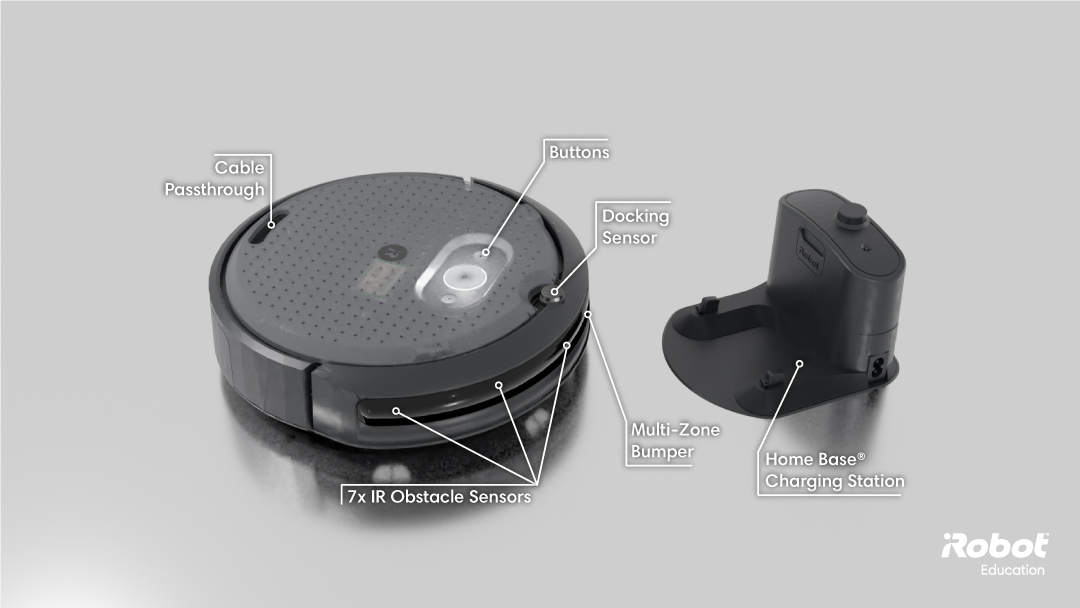
\includegraphics[width=0.8\linewidth]{figures/irobot_create_3}
	\caption[Overview of the iRobot® Create® 3]{Overview of the iRobot® Create® 3}
	\label{fig:irobot_create_3}
\end{figure}

The software ecosystem of the Create 3 base is natively integrated with ROS 2. Sensor telemetry is broadcast continuously via ROS 2 publishers, while internal actuators are controlled, and user commands processed, through standardized ROS 2 subscribers and service servers. Furthermore, the base features pre-programmed autonomous behaviors out of the box, including automated docking, wall-following, and reactive obstacle avoidance. These behaviors can be dynamically triggered, monitored, and adjusted utilizing ROS 2 actions and parameters.

The user interface on the top surface of the base consists of three physical buttons and a centralized LED light ring.

\begin{figure}[!ht]
	\centering
	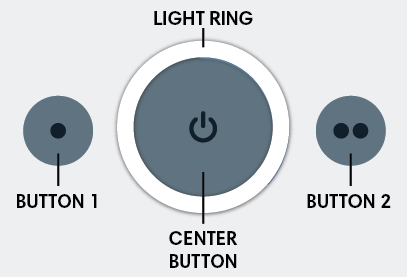
\includegraphics[width=0.7\linewidth]{figures/iRobot_Create_Buttons}
	\caption[Buttons and Light ring on the Base]{Buttons and Light ring configuration on the iRobot Create 3 base and its docking station}
	\label{fig:irobotcreatebuttons}
\end{figure}

The primary center button, marked with a power icon, manages the operational state (power on/off) of the base. The two adjacent, smaller buttons can be mapped to custom user-defined software callbacks. The surrounding LED light ring functions as a visual telemetry indicator, communicating distinct operational states such as active charging, idle standby, system warnings, or critical hardware errors. For exhaustive diagnostics regarding these illumination patterns, the official documentation should be consulted. Additionally, the base includes an autonomous charging dock, allowing the robot to navigate and attach itself independently to replenish its battery.

\newpage

\subsection{Standard Onboard Sensors}
For basic navigation, environmental mapping, and safety enforcement, the TurtleBot 4 relies on a combination of tactile, inertial, and laser-based sensors. The primary payload is the RPLIDAR A1M8 sensor, a 2D LiDAR (Light Detection and Ranging) scanner, mounted on the top deck. This sensor performs continuous 360-degree planar scans of the surrounding environment, generating precise distance measurements that are highly critical for Simultaneous Localization and Mapping (SLAM) and real-time obstacle avoidance.

\begin{figure}[!ht]
	\centering
	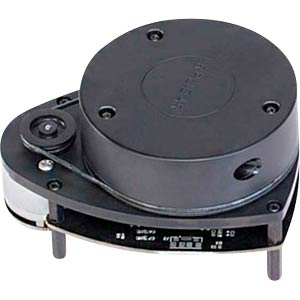
\includegraphics[width=0.5\linewidth]{figures/RPLIDAR_A1M8_sensor.png}
	\caption[RPLIDAR A1M8 LiDAR scanner]{RPLIDAR A1M8 360° Laser Scanner}
	\label{fig:lidar_sensor}
\end{figure}

Odometry tracking is achieved through high-resolution optical wheel encoders working in tandem with an Inertial Measurement Unit (IMU). The wheel encoders measure the exact rotations of the drive wheels to calculate the robot's relative position and velocity over time. The IMU supplements this data by measuring angular velocity and linear acceleration, improving orientation tracking. To ensure operational safety, the front of the iRobot Create 3 base is equipped with a mechanical bumper sensor. This tactile sensor serves as a physical fail-safe; upon physical contact with an object, it instantly triggers a safety interrupt via ROS 2 to halt the actuators, preventing potential damage from obstacles missed by the primary rangefinders.

\subsection{The Luxonis OAK-D Pro Spatial Camera}
For advanced computer vision perception, the TurtleBot 4 is equipped with a Luxonis OAK-D Pro hardware camera module. Structurally, the OAK-D Pro is designed as an all-in-one spatial AI camera platform featuring an onboard Visual Processing Unit (VPU). While this built-in architecture is theoretically capable of executing deep learning neural networks directly on the edge to offload processing tasks from a host system, utilizing the internal VPU for real-time inference was out of scope due to the development timeline constraints of this project.

\begin{figure}[!ht]
	\centering
	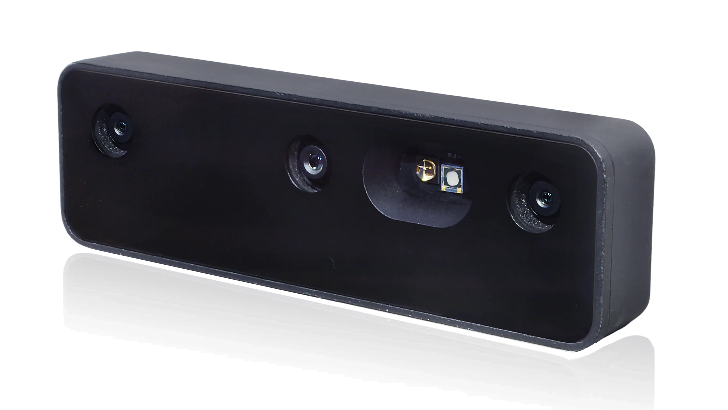
\includegraphics[width=0.6\linewidth]{figures/oakd_pro_camera.png}
	\caption[Luxonis OAK-D Pro Camera]{The Luxonis OAK-D Pro spatial depth camera mounted on the platform.}
	\label{fig:oakd_camera}
\end{figure}

Instead of leveraging the camera's local edge-computing unit, this thesis utilizes the platform as a highly synchronized, raw spatial sensor array. The camera system features a trinocular configuration to gather comprehensive environmental data. It combines two global-shutter monochrome cameras to calculate stereo depth perception with a centralized high-resolution RGB color camera optimized for feature tracking and object classification. 

In the physical hardware configuration of the TurtleBot 4, these heterogeneous image matrices — specifically the synchronized color and stereo depth data streams — are transmitted natively via a physical USB 3.0 interface directly to the onboard Raspberry Pi 4 processing unit. This high-bandwidth connection ensures that the raw sensory data is delivered to the robot's local computing layer with minimal hardware latency. Additionally, the camera features an integrated infrared illumination system, incorporating a dot projector and a flood LED. This configuration enables reliable depth sensing and surface tracking capabilities even in low-light or zero-light laboratory environments, providing a robust stream of spatial information to the robot's primary interface.


\section{ROS2} % ----------------------------------------------------------------
The Robot Operating System (ROS) is a comprehensive set of open-source software libraries and tools designed to facilitate the development of applications for robotic systems. It includes a wide variety of drivers for state-of-the-art algorithms, graphical user interface (GUI) development tools, and extensive resources suitable for any type of robotics project. 

\begin{figure}[!ht]
	\centering
	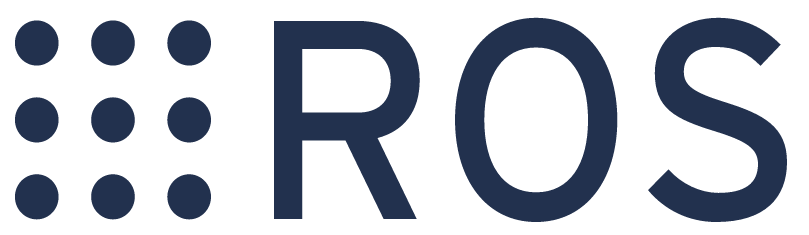
\includegraphics[width=0.6\linewidth]{figures/Ros_logo.png}
	\caption[ROS 2 Logo]{ROS 2 Logo}
	\label{fig:ros2}
\end{figure}

Fundamentally, ROS operates as the architectural glue of the entire robotic system. Instead of a monolithic software structure, the developer implements modular components known as nodes to add specific functionalities or support for particular hardware. These nodes communicate with one another asynchronously or synchronously through dedicated mechanisms: topics, services, or actions. Because the communication messages within ROS are strictly standardized, the framework is inherently language-agnostic. Nodes can be developed in different programming languages, provided their inputs and outputs comply with the defined message structures. Consequently, a developer might implement a low-level motor driver in C++ to achieve optimal hardware performance, while simultaneously utilizing Python for high-level image recognition programs or neural networks.

While the framework is commonly referred to simply as ROS, there are actually two distinct generations, known as ROS1 and ROS2 respectively. The first version, ROS1, entered development in 2007 by a company called Willow Garage, originating from a university project at Stanford University. Its first official release was published in March 2010. While this version proved highly successful by introducing features such as a peer-to-peer architecture, computational modularity, and widespread code reusability, it possessed inherent limitations. These included a single point of failure within its centralized ROS Master system, a lack of deterministic real-time support, poor Wi-Fi integration, and no native support for multi-robot setups.

To address these commercial and architectural limitations, the development of ROS2 began in 2014. With its first official alpha release in 2015, a fundamentally redesigned iteration of the framework was introduced. These improvements replaced the legacy ROS Master with an industry-standard Data Distribution Service (DDS) middleware, successfully eliminating the single point of failure. Furthermore, ROS2 introduced native support for real-time execution, robust multi-robot communication, and Quality of Service (QoS) profiles. The latter is highly critical for high-bandwidth data management, such as handling live video streams. Ultimately, these advancements significantly streamlined industrial-grade deployment.
 


\section{YOLO} % -------------------------------------------------------------

The computer vision framework selected for the practical implementation of this thesis is YOLO (an acronym for "You Only Look Once"), specifically the modern iterations maintained by the company Ultralytics. Originally introduced by Joseph Redmon et al. in 2015, the YOLO architecture revolutionized the field of computer vision. Unlike traditional regional-based convolutional neural networks (R-CNNs) that require a two-stage process for region proposal and classification, YOLO frames object detection as a single regression problem. By processing the entire image through a single neural network in a single forward pass, it achieves exceptional inference speeds, making it the premier choice for real-time robotic vision applications.

\begin{figure}[!ht]
	\centering
	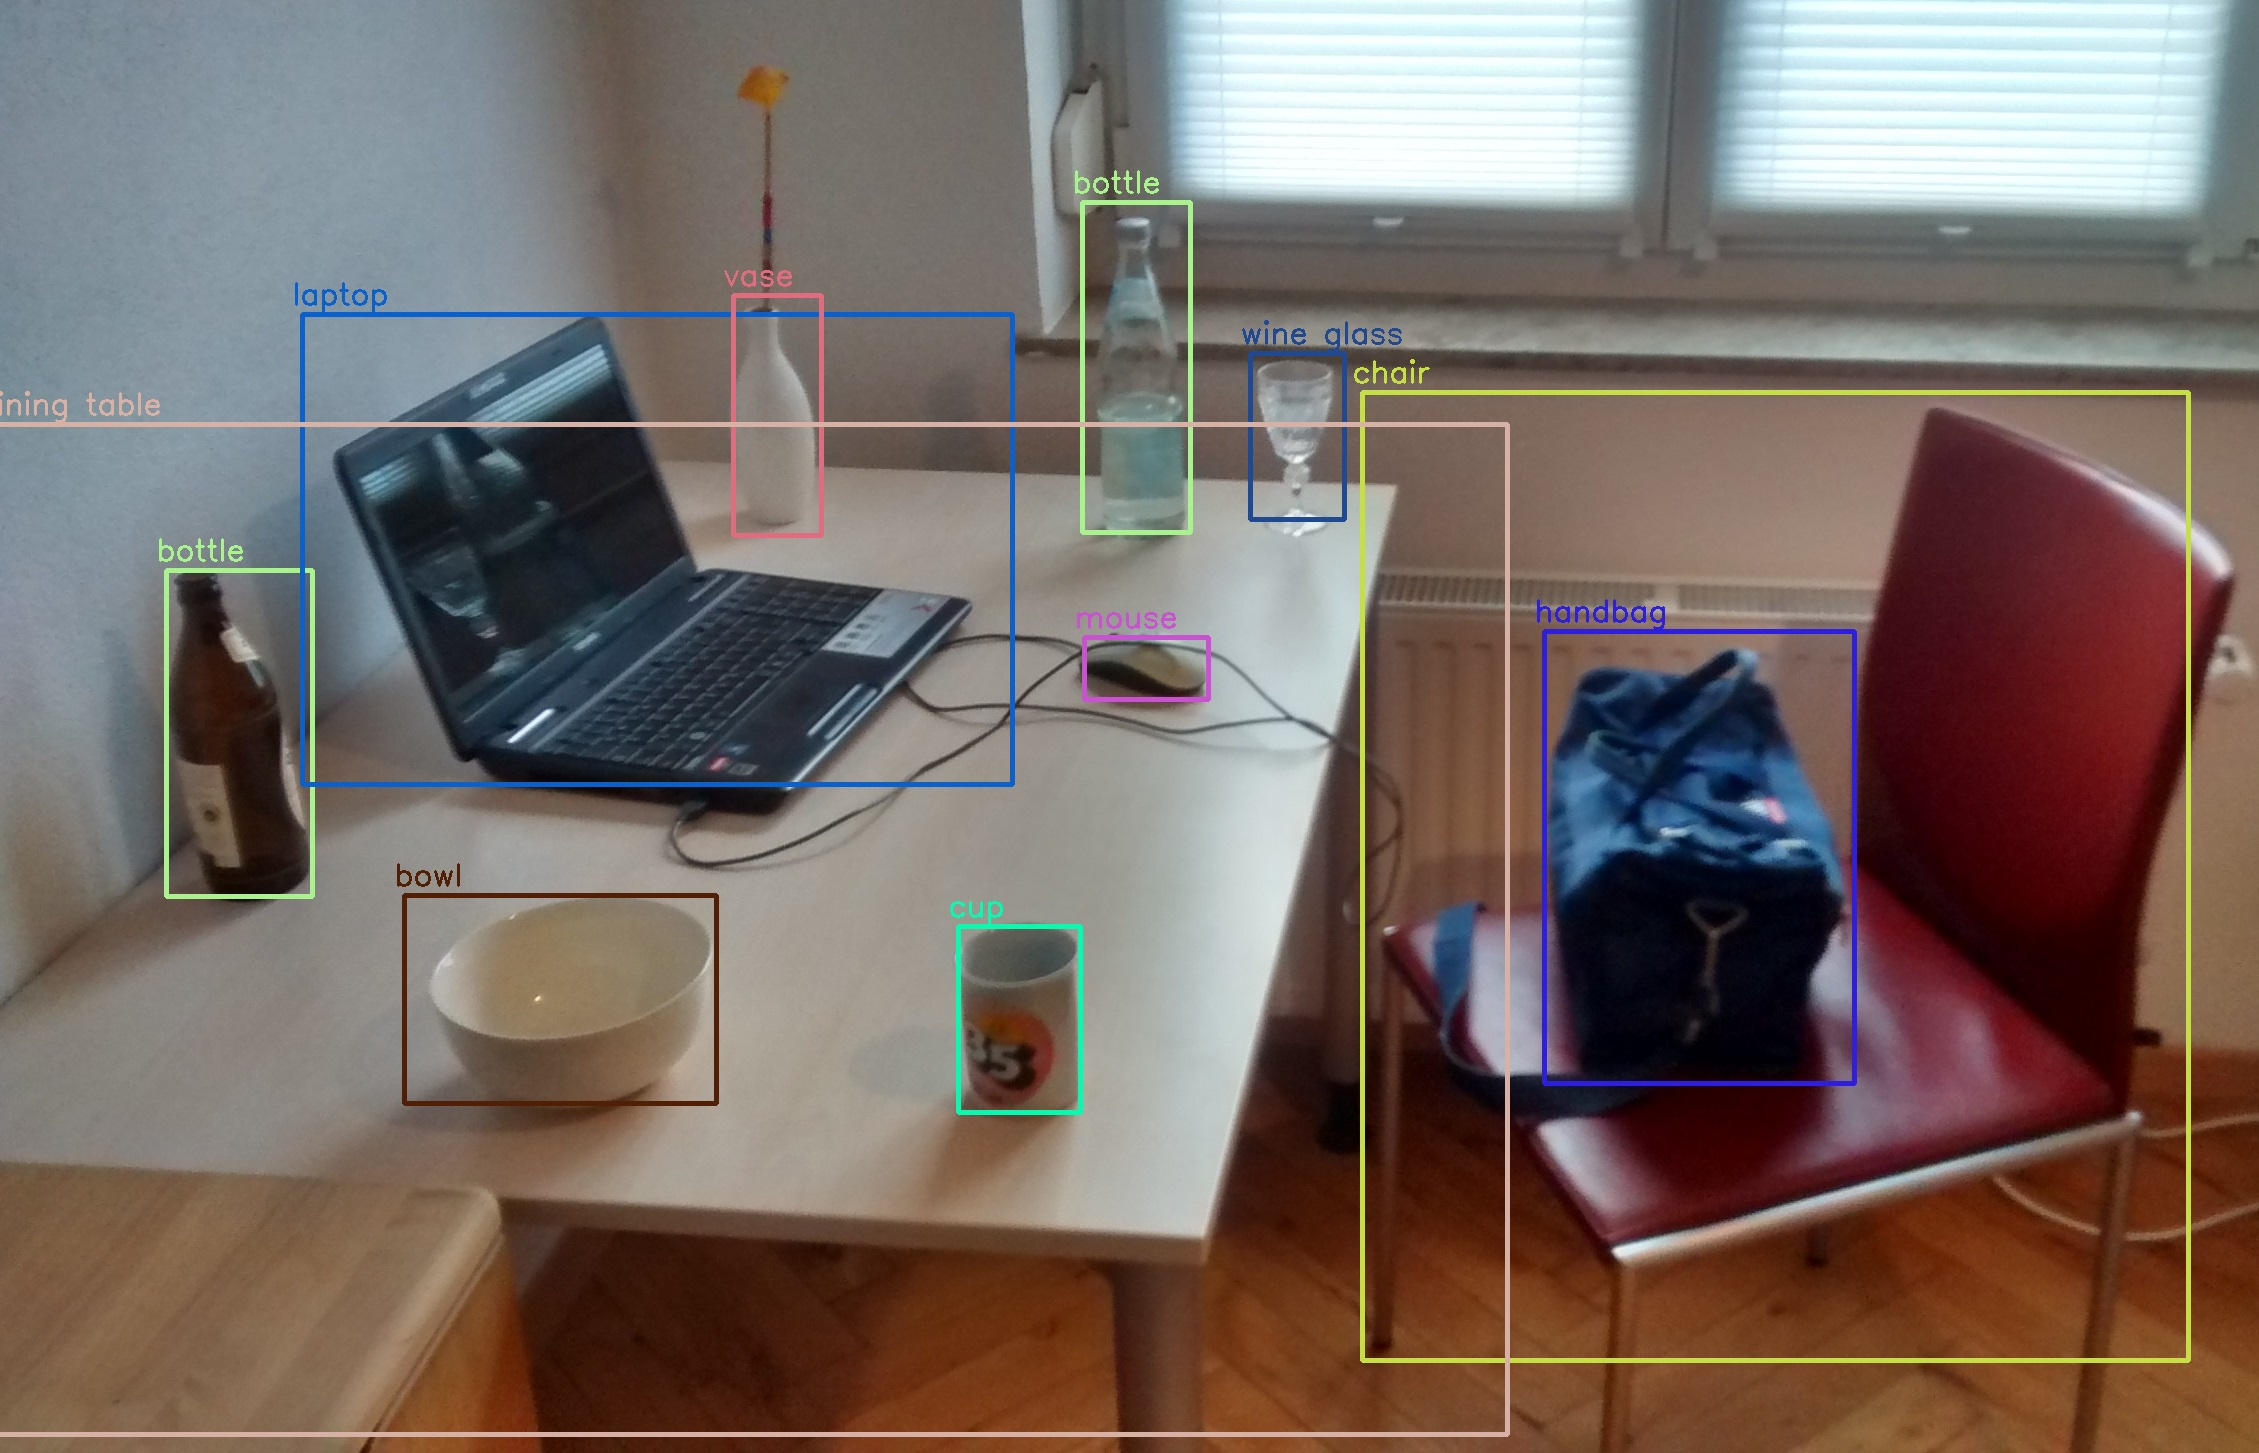
\includegraphics[width=0.6\linewidth]{figures/YOLO_detecting_objects.png}
	\caption[YOLO detecting Objects]{YOLO detecting Objects with the COCO dataset}
	\label{fig:yolo}
\end{figure}

In modern robotics pipelines, Ultralytics' deployment of YOLO has become the industry standard due to its balance between computational efficiency and high precision. The framework provides robust pretrained models that have been optimized using benchmarks trained on millions of labeled images, such as the COCO (Common Objects in Context) dataset. For rapid prototyping and seamless software integration, it features a native Python module. Furthermore, the architecture is highly scalable, offering various model scales ranging from "nano" ($n$) for resource-constrained edge devices like the Raspberry Pi, up to "extra-large" ($x$) for high-performance workstation GPUs. 

Beyond standard object detection (generating 2D bounding boxes), modern versions of YOLO have evolved into comprehensive multi-task vision frameworks. They natively support instance segmentation (pixel-level masking), object tracking across sequential video frames, and pose estimation (keypoint detection). This versatility allows the robotic system to not only identify and locate obstacles or targets but also to understand their orientation, motion vectors, and precise geometry within the environment.
